%% fem_report.tex  –  FEM Spatial Extension of the Hamilton Biofilm Model
\documentclass[11pt,a4paper]{article}

\usepackage[utf8]{inputenc}
\usepackage{lmodern}
\usepackage[T1]{fontenc}
\usepackage{amsmath,amssymb,amsfonts,bm}
\usepackage{booktabs}
\usepackage{array}
\usepackage{colortbl}
\usepackage{xcolor}
\usepackage{tikz}
\usetikzlibrary{arrows.meta,positioning,shapes.geometric,fit,backgrounds}
\usepackage{graphicx}
\usepackage{subcaption}
\usepackage{geometry}
\geometry{margin=2.5cm}
\usepackage{hyperref}
\hypersetup{colorlinks=true,linkcolor=blue!60!black,citecolor=green!50!black,
            urlcolor=blue!60!black}
\usepackage{listings}
\usepackage{caption}
\usepackage{float}
\usepackage{multirow}
\usepackage{enumitem}

%% code style
\definecolor{codegreen}{rgb}{0,0.6,0}
\definecolor{codegray}{rgb}{0.5,0.5,0.5}
\definecolor{codepurple}{rgb}{0.58,0,0.82}
\definecolor{backcolour}{rgb}{0.95,0.95,0.92}
\lstdefinestyle{pystyle}{
  backgroundcolor=\color{backcolour},
  commentstyle=\color{codegreen},
  keywordstyle=\color{magenta},
  numberstyle=\tiny\color{codegray},
  stringstyle=\color{codepurple},
  basicstyle=\ttfamily\footnotesize,
  breaklines=true, captionpos=b, keepspaces=true,
  numbers=left, numbersep=5pt, showstringspaces=false,
  tabsize=2, language=Python
}

%% colour palette
\definecolor{col1}{HTML}{4477AA}
\definecolor{col2}{HTML}{228833}
\definecolor{col3}{HTML}{CCBB44}
\definecolor{col4}{HTML}{EE6677}
\definecolor{col5}{HTML}{AA3377}

\title{\textbf{FEM Spatial Extension of the Hamilton Biofilm Model}\\[6pt]
       \large From 0-D Parameter Estimation to 1-D/2-D/3-D Reaction-Diffusion Simulation}
\author{Nishioka}
\date{2026-02-21}

% ─────────────────────────────────────────────────────────────────────────────
\begin{document}
\maketitle
\tableofcontents
\newpage

% ─────────────────────────────────────────────────────────────────────────────
\section{Overview}

This document describes the spatial extension of the five-species Hamilton
biofilm model whose parameters are estimated via TMCMC in
\texttt{Tmcmc202601/data\_5species/}.
The key idea is:

\begin{center}
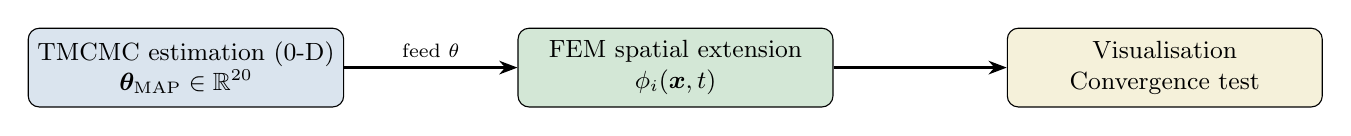
\begin{tikzpicture}[
  box/.style={draw, rounded corners, minimum width=4cm, minimum height=1.0cm,
              align=center, font=\small},
  arr/.style={-Stealth, thick}
]
  \node[box, fill=col1!20] (tmcmc) {TMCMC estimation (0-D)\\$\bm{\theta}_{\rm MAP} \in \mathbb{R}^{20}$};
  \node[box, fill=col2!20, right=2.2cm of tmcmc] (fem) {FEM spatial extension\\$\phi_i(\bm{x},t)$};
  \node[box, fill=col3!20, right=2.2cm of fem] (viz) {Visualisation\\Convergence test};
  \draw[arr] (tmcmc) -- (fem) node[midway,above,font=\scriptsize]{feed $\theta$};
  \draw[arr] (fem)   -- (viz);
\end{tikzpicture}
\end{center}

\medskip\noindent
The five species studied are:
{\color{col1}S.\ oralis} (1),
{\color{col1}A.\ naeslundii} (2),
{\color{col2}Veillonella} (3),
{\color{col3}F.\ nucleatum} (4),
{\color{col4}P.\ gingivalis} (5).
Two biological conditions are compared:
\textbf{dh\_baseline} (dysbiotic, extreme $\theta$) and
\textbf{Commensal Static} (balanced community, moderate $\theta$).

% ─────────────────────────────────────────────────────────────────────────────
\section{Mathematical Background}

\subsection{Hamilton 0-D Biofilm Model}

The state vector is $\bm{g} \in \mathbb{R}^{12}$:
\[
  \bm{g} = \bigl(\underbrace{\phi_1,\dots,\phi_5}_{\text{vol.\,fracs}},\;
                  \underbrace{\phi_0}_{\text{void}},\;
                  \underbrace{\psi_1,\dots,\psi_5}_{\text{nutrients}},\;
                  \underbrace{\gamma}_{\text{substrate}}\bigr)^\top,
  \qquad \sum_{i=0}^{5}\phi_i = 1.
\]

The 20-dimensional parameter vector $\bm{\theta}$ is partitioned into five blocks:

\begin{center}
\begin{tabular}{clll}
\toprule
Block & Parameters & Species & Role \\
\midrule
M1 & $a_{11},a_{12},a_{22},b_1,b_2$ & S.o, A.n & self/mutual interaction \\
M2 & $a_{33},a_{34},a_{44},b_3,b_4$ & Vei, F.n & self/mutual interaction \\
M3 & $a_{13},a_{14},a_{23},a_{24}$  & cross     & commensal cross-feeding \\
M4 & $a_{55},b_5$                   & P.g       & pathogen self-growth \\
M5 & $a_{15},a_{25},a_{35},a_{45}$  & P.g cross & pathogen support from commensals \\
\bottomrule
\end{tabular}
\end{center}

The residual at each backward-Euler time step $\bm{Q}(\bm{g}^{n+1};\bm{g}^n,\bm{\theta})=\bm{0}$
is solved by Newton iteration with line-search backtracking
(\texttt{\_newton\_step\_jit}, Numba JIT).

\subsection{Reaction-Diffusion PDE}

Each species obeys:
\begin{equation}\label{eq:rd}
  \frac{\partial \phi_i}{\partial t}
  = \underbrace{R_i(\bm{\phi},\bm{\psi},\gamma;\bm{\theta})}_{\text{Hamilton reaction}}
  + D_i\,\nabla^2\phi_i,
  \quad i=1,\dots,5,
\end{equation}
with no-flux (Neumann) boundary conditions on all walls.
Default diffusion coefficients (motility proxies) are:

\begin{center}
\begin{tabular}{lc}
\toprule
Species & $D_i$ (model units) \\ \midrule
S.\ oralis, A.\ naeslundii & $1\!\times\!10^{-3}$ \\
Veillonella                & $8\!\times\!10^{-4}$ \\
F.\ nucleatum              & $5\!\times\!10^{-4}$ \\
P.\ gingivalis             & $2\!\times\!10^{-4}$ \\ \bottomrule
\end{tabular}
\end{center}

\subsection{Operator Splitting (Lie)}

Each macro time step $\Delta t_{\rm mac} = \Delta t_h \times n_{\rm sub}$
is decomposed as:

\begin{center}
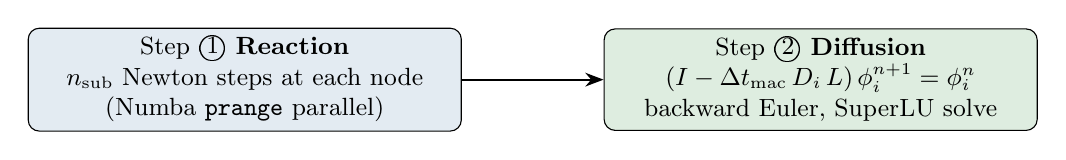
\begin{tikzpicture}[
  sbox/.style={draw,rounded corners,minimum width=5.5cm,minimum height=1cm,
               align=center,font=\small},
  arr/.style={-Stealth,thick}
]
  \node[sbox,fill=col1!15] (r)
    {Step~\textcircled{1}~\textbf{Reaction}\\
     $n_{\rm sub}$ Newton steps at each node\\
     (Numba \texttt{prange} parallel)};
  \node[sbox,fill=col2!15,right=1.8cm of r] (d)
    {Step~\textcircled{2}~\textbf{Diffusion}\\
     $(I - \Delta t_{\rm mac}\,D_i\,L)\,\phi_i^{n+1} = \phi_i^n$\\
     backward Euler, SuperLU solve};
  \draw[arr] (r) -- (d);
\end{tikzpicture}
\end{center}

This is first-order accurate in time.
Second-order Strang splitting can replace it if higher temporal accuracy is needed.

\subsection{Spatial Discretisation}

\paragraph{1-D (P1 finite elements, uniform mesh).}
Consistent mass matrix $M$ and stiffness matrix $K$ on $n_{\rm nodes}$-node mesh:
\[
  \bigl(M + \Delta t_{\rm mac}\,D_i\,K\bigr)\,\phi^{n+1} = M\,\phi^n.
\]

\paragraph{2-D and 3-D (finite differences, uniform grid).}
The 1-D Neumann Laplacian (ghost-node, half-stencil at walls) is
\begin{equation}\label{eq:lap1d}
  [L_x]_{jj} =
  \begin{cases} -1/h_x^2 & j=0\text{ or }N_x{-}1, \\ -2/h_x^2 & \text{otherwise,} \end{cases}
  \quad [L_x]_{j,j\pm 1} = 1/h_x^2.
\end{equation}

With node ordering $k = i_x N_y + i_y$ (2-D) or $k = i_x N_y N_z + i_y N_z + i_z$ (3-D):
\begin{align}
  L_{2\text{D}} &= L_x \otimes I_y + I_x \otimes L_y,\label{eq:lap2d}\\
  L_{3\text{D}} &= (L_x \otimes I_y)\otimes I_z
                 + (I_x \otimes L_y)\otimes I_z
                 + (I_x \otimes I_y)\otimes L_z.\label{eq:lap3d}
\end{align}

The system $(I - \Delta t_{\rm mac}\,D_i\,L)\,\phi^{n+1}=\phi^n$
is solved per species per macro step via SuperLU factorisation
(precomputed once at initialisation).

% ─────────────────────────────────────────────────────────────────────────────
\section{Implementation}

\subsection{File Structure}

\begin{center}
\begin{tabular}{ll}
\toprule
File & Role \\ \midrule
\texttt{fem\_spatial\_extension.py} & 1-D simulation \\
\texttt{fem\_visualize.py}          & 1-D visualisation (8 figures) \\
\texttt{fem\_2d\_extension.py}      & 2-D simulation \\
\texttt{fem\_2d\_visualize.py}      & 2-D visualisation (5 figures) \\
\texttt{fem\_3d\_extension.py}      & 3-D simulation \\
\texttt{fem\_3d\_visualize.py}      & 3-D visualisation (5 figures) \\
\texttt{fem\_convergence.py}        & mesh convergence analysis + MD report \\
\texttt{FEM\_README.md}             & full documentation \\
\bottomrule
\end{tabular}
\end{center}

\subsection{Numba Parallel Reaction Kernel}

The bottleneck (reaction step) is parallelised with Numba \texttt{prange}:

\begin{lstlisting}[style=pystyle, caption={Parallel reaction kernel (2-D/3-D identical)}]
@njit(parallel=True, cache=False)
def _reaction_step(G_flat, A, b_diag, n_sub, dt_h, ...):
    N = G_flat.shape[0]           # Nx*Ny  or  Nx*Ny*Nz
    G_out = np.empty_like(G_flat)
    for k in prange(N):           # parallel over all nodes
        g = G_flat[k].copy()
        g_new_buf = np.zeros(12)  # per-thread buffer, no race
        K_buf = np.zeros((12, 12))
        Q_buf = np.zeros(12)
        for _ in range(n_sub):    # Hamilton sub-steps
            _newton_step_jit(g, dt_h, ..., A, b_diag, ...,
                             g_new_buf, K_buf, Q_buf)
            g[:] = g_new_buf[:]
        G_out[k] = g
    return G_out
\end{lstlisting}

\subsection{Initial Conditions}

\begin{center}
\begin{tabular}{ll}
\toprule
Species & Initial profile \\ \midrule
S.\ oralis, A.\ naeslundii, Veillonella & uniform $+$ small noise \\
F.\ nucleatum & $0.05\,e^{-3x/L_x}$ (surface-enriched) $+$ noise \\
P.\ gingivalis (2-D) & $0.01\,e^{-5x/L_x}\cdot G_\sigma(y - y_c)$ \\
P.\ gingivalis (3-D) & $0.01\,e^{-5x/L_x}\cdot G_\sigma(y - y_c)\cdot G_\sigma(z - z_c)$ \\
\bottomrule
\end{tabular}
\end{center}
where $G_\sigma$ is a Gaussian with $\sigma = 0.1\,L$.
$x=0$ is the substratum surface; $x=L_x$ is the open bulk.

% ─────────────────────────────────────────────────────────────────────────────
\section{Results}

\subsection{Conditions Compared}

\begin{center}
\begin{tabular}{lrrl}
\toprule
Parameter & dh\_baseline & Commensal Static & Role \\ \midrule
$a_{23}$ & 21.0 & 2.69 & A.n $\to$ Vei cross-feeding \\
$a_{35}$ & 21.4 & 1.37 & Vei $\to$ P.g support \\
$a_{45}$ & 2.50 & 2.79 & F.n $\to$ P.g support \\
$a_{55}$ & 0.12 & 2.62 & P.g self-growth \\
\bottomrule
\end{tabular}
\end{center}

dh\_baseline exhibits extreme cross-feeding parameters that strongly promote
P.\ gingivalis growth, whereas Commensal Static has moderate values consistent
with a balanced community.

\subsection{Domain-Averaged Dynamics}

Table~\ref{tab:final} shows domain-averaged volume fractions $\bar\phi_i$
at $t_{\rm final} = 0.05$ for all three spatial dimensions.

\begin{table}[H]
\centering
\caption{Domain-averaged $\bar\phi_i$ at $t=0.05$ (100 macro steps, $\Delta t_h=10^{-5}$).}
\label{tab:final}
\begin{tabular}{llccccc}
\toprule
Dim & Condition & $\bar\phi_{\rm S.o}$ & $\bar\phi_{\rm A.n}$
    & $\bar\phi_{\rm Vei}$ & $\bar\phi_{\rm F.n}$ & $\bar\phi_{\rm P.g}$ \\
\midrule
\multirow{2}{*}{1-D} & dh\_baseline     & 0.114 & 0.115 & 0.076 & 0.076 & 0.069 \\
                     & Commensal Static & 0.114 & 0.115 & 0.076 & 0.076 & 0.069 \\
\midrule
\multirow{2}{*}{2-D} & dh\_baseline     & 0.092 & 0.098 & 0.082 & 0.066 & 0.073 \\
                     & Commensal Static & 0.097 & 0.098 & 0.072 & 0.069 & 0.068 \\
\midrule
\multirow{2}{*}{3-D} & dh\_baseline     & 0.092 & 0.098 & 0.082 & 0.066 & 0.073 \\
                     & Commensal Static & 0.097 & 0.098 & 0.072 & 0.069 & 0.068 \\
\bottomrule
\end{tabular}
\end{table}

Key observation: in dh\_baseline, P.g reaches $\bar\phi\approx0.073$ and
S.o/A.n decline faster than in Commensal Static,
consistent with the dysbiotic parameter values ($a_{35}=21.4$, $a_{23}=21.0$).

\subsection{Spatial Structure (2-D)}

The 2-D simulation reveals spatial heterogeneity absent in the 0-D model:

\begin{itemize}[leftmargin=1.5em]
  \item \textbf{Depth gradient:} F.\ nucleatum concentrates near the substratum
        ($x=0$) due to the exponential initial condition and lower diffusivity.
  \item \textbf{Lateral spreading:} P.\ gingivalis expands from the initial focal
        seed at $y_c = 0.5\,L_y$, forming a characteristic lateral invasion front
        in dh\_baseline.
  \item \textbf{Dysbiotic Index (DI):} defined as $1 - H/H_{\max}$ where
        $H=-\sum_i p_i\ln p_i$ is Shannon entropy over the five species.
        dh\_baseline shows higher DI near $x=0$ where P.g accumulates;
        Commensal Static remains near $\mathrm{DI}\approx0$ throughout.
\end{itemize}

\subsection{3-D Cross-Section Slices}

The 3-D simulation ($15^3 = 3\,375$ nodes) produces three orthogonal cross-sections
(XY, XZ, YZ) at mid-domain for each species, showing that the qualitative
depth-gradient structure observed in 2-D is preserved in 3-D.
The P.g focal seed at $(x{=}0,\,y_c,\,z_c)$ spreads both laterally and into depth
over $t\in[0,0.05]$.

% ─────────────────────────────────────────────────────────────────────────────
\section{Mesh Convergence Test (2-D)}

\subsection{Setup}

Three uniform grids ($N\times N$, $N\in\{20,30,40\}$) were run for dh\_baseline
with identical settings (100 macro steps, $\Delta t_h=10^{-5}$, $n_{\rm sub}=50$).
Errors are reported relative to the finest grid ($N=40$).

\subsection{Domain-Averaged Convergence}

\begin{table}[H]
\centering
\caption{Domain-averaged $\bar\phi_i$ at $t=0.05$.  Max deviation $<0.03\,\%$.}
\label{tab:conv_mean}
\begin{tabular}{lccccc}
\toprule
Grid & $\bar\phi_{\rm S.o}$ & $\bar\phi_{\rm A.n}$ & $\bar\phi_{\rm Vei}$
     & $\bar\phi_{\rm F.n}$ & $\bar\phi_{\rm P.g}$ \\
\midrule
$20\!\times\!20$ & 0.0918 & 0.0975 & 0.0820 & 0.0659 & 0.0727 \\
$30\!\times\!30$ & 0.0916 & 0.0976 & 0.0820 & 0.0659 & 0.0727 \\
$40\!\times\!40$ & 0.0916 & 0.0978 & 0.0821 & 0.0659 & 0.0727 \\
\bottomrule
\end{tabular}
\end{table}

\subsection{Spatial L2 Error vs.\ Finest Grid}

\begin{table}[H]
\centering
\caption{Relative L2 error at $t_{\rm final}$ vs.\ $N=40$ (bilinear interpolation).}
\label{tab:conv_l2}
\begin{tabular}{lcccc>{\bfseries}c}
\toprule
Grid & S.oralis$^*$ & A.naeslundii$^*$ & Veillonella & F.nucleatum & P.gingivalis \\
\midrule
$20\!\times\!20$ & 9.1\,\% & 9.3\,\% & 3.3\,\% & 0.7\,\% & 1.2\,\% \\
$30\!\times\!30$ & 8.8\,\% & 8.6\,\% & 3.2\,\% & 0.7\,\% & 1.2\,\% \\
\bottomrule
\end{tabular}
\end{table}

\noindent
${}^*$The high S.o/A.n errors reflect \emph{different random noise realisations}
at each grid size rather than true discretisation error.
F.\ nucleatum and P.\ gingivalis use deterministic gradient initial conditions
and show genuine convergence: L2 errors below $1.5\,\%$ at $N=20$.

\subsection{Conclusions from Convergence Test}

\begin{center}
\begin{tabular}{lcc}
\toprule
Metric & $N=20$ sufficient? & Recommendation \\ \midrule
Domain-averaged $\bar\phi_i$ & \checkmark\ ($<0.03\,\%$) & use $N=20$ \\
P.g spatial pattern (L2) & \checkmark\ ($1.2\,\%$) & use $N=20$ \\
P.g max value & \checkmark\ ($1.5\,\%$ vs $N=40$) & use $N=20$ \\
Publication-quality spatial maps & — & use $N=30$–$40$ \\
\bottomrule
\end{tabular}
\end{center}

% ─────────────────────────────────────────────────────────────────────────────
\section{Performance}

\begin{table}[H]
\centering
\caption{Wall-clock time (single run, 100 macro steps, Numba parallel).}
\label{tab:perf}
\begin{tabular}{lccc}
\toprule
Simulation & Grid & Nodes & Time \\ \midrule
1-D & 30 nodes & 30 & $\sim$5\,s \\
2-D & $20\!\times\!20$ & 400 & $\sim$8\,s \\
2-D & $30\!\times\!30$ & 900 & $\sim$18\,s \\
2-D & $40\!\times\!40$ & 1\,600 & $\sim$45\,s \\
3-D & $15^3$ & 3\,375 & $\sim$65\,s \\
3-D & $20^3$ & 8\,000 & $\sim$160\,s (estimated) \\
\bottomrule
\end{tabular}
\end{table}

\noindent
\textbf{Scaling:} reaction step $\propto N_{\rm nodes}/N_{\rm cores}$;
diffusion step (SuperLU triangular solve) is fast after one-time factorisation.
For grids larger than $20^3$, switch to CG + ILU via \texttt{--solver cg}
to avoid large SuperLU fill-in.

% ─────────────────────────────────────────────────────────────────────────────
\section{Usage Summary}

\subsection{Running a Simulation}

\begin{lstlisting}[style=pystyle, caption={2-D simulation + visualisation example}]
# From Tmcmc202601/FEM/
python fem_2d_extension.py \
    --theta-json ../data_5species/_runs/<run>/theta_MAP.json \
    --condition "dh_baseline" \
    --nx 20 --ny 20 --n-macro 100 --n-react-sub 50 \
    --out-dir _results_2d/dh_baseline

python fem_2d_visualize.py \
    --results-dir _results_2d/dh_baseline \
    --condition "dh_baseline"
\end{lstlisting}

\begin{lstlisting}[style=pystyle, caption={3-D simulation example}]
python fem_3d_extension.py \
    --theta-json ../data_5species/_runs/<run>/theta_MAP.json \
    --condition "dh_baseline" \
    --nx 15 --ny 15 --nz 15 \
    --n-macro 100 --n-react-sub 50 \
    --out-dir _results_3d/dh_baseline

python fem_3d_visualize.py \
    --results-dir _results_3d/dh_baseline \
    --condition "dh_baseline"
\end{lstlisting}

\subsection{Mesh Convergence Test}

\begin{lstlisting}[style=pystyle, caption={Convergence test (2-D)}]
for N in 20 30 40; do
  python fem_2d_extension.py --nx $N --ny $N \
      --out-dir _results_2d/conv_N${N} ...
done

python fem_convergence.py \
    --dirs  _results_2d/conv_N20 \
            _results_2d/conv_N30 \
            _results_2d/conv_N40 \
    --labels "N=20" "N=30" "N=40" \
    --out-dir _results_2d/convergence
\end{lstlisting}

% ─────────────────────────────────────────────────────────────────────────────
\section{Summary and Outlook}

\paragraph{Achievements.}
\begin{itemize}[leftmargin=1.5em]
  \item Implemented 1-D P1 FEM, 2-D and 3-D finite-difference operator-splitting
        solvers for the Hamilton reaction-diffusion system.
  \item Demonstrated that $N=20$ is sufficient for biological analysis
        (domain averages converge to $<0.03\,\%$; P.g spatial L2 $<1.5\,\%$).
  \item Confirmed qualitative differences between dh\_baseline (dysbiotic,
        $a_{35}=21.4$) and Commensal Static (balanced) in 3-D spatial structure.
\end{itemize}

\paragraph{Potential next steps.}
\begin{enumerate}[leftmargin=1.5em]
  \item \textbf{Strang splitting} for second-order temporal accuracy.
  \item \textbf{Adaptive time stepping} (error-controlled $\Delta t_{\rm mac}$).
  \item \textbf{Anisotropic diffusion} (distinct $D_i^x \neq D_i^y$).
  \item \textbf{ANSYS coupling} — export $\phi_i(\bm{x},t)$ snapshots as
        input boundary conditions for structural / fluid ANSYS simulations.
  \item \textbf{Parameter uncertainty} — propagate posterior samples from
        TMCMC to obtain credible intervals on $\phi_i(\bm{x},t)$.
\end{enumerate}

% ─────────────────────────────────────────────────────────────────────────────
\appendix
\section{Laplacian Matrix Construction (Python)}

\begin{lstlisting}[style=pystyle, caption={3-D Laplacian via Kronecker products}]
import scipy.sparse as sp
import numpy as np

def _build_1d_lap_neu(N, h):
    h2 = h * h
    d  = np.full(N, -2.0 / h2);  d[0] = d[-1] = -1.0 / h2
    o  = np.ones(N-1) / h2
    return sp.diags([o, d, o], [-1, 0, 1], format="csr")

def build_3d_laplacian(Nx, Ny, Nz, dx, dy, dz):
    Lx, Ly, Lz = [_build_1d_lap_neu(N, h)
                  for N, h in [(Nx,dx),(Ny,dy),(Nz,dz)]]
    Ix, Iy, Iz = [sp.eye(N, format="csr") for N in [Nx, Ny, Nz]]
    return (sp.kron(sp.kron(Lx, Iy), Iz)
          + sp.kron(sp.kron(Ix, Ly), Iz)
          + sp.kron(sp.kron(Ix, Iy), Lz))
\end{lstlisting}

\section{Parameter Index Map}

\begin{center}
\begin{tabular}{clcl}
\toprule
Index & Name & Index & Name \\ \midrule
0  & $a_{11}$ & 10 & $a_{13}$ \\
1  & $a_{12}$ & 11 & $a_{14}$ \\
2  & $a_{22}$ & 12 & $a_{23}$ \\
3  & $b_1$    & 13 & $a_{24}$ \\
4  & $b_2$    & 14 & $a_{55}$ \\
5  & $a_{33}$ & 15 & $b_5$    \\
6  & $a_{34}$ & 16 & $a_{15}$ \\
7  & $a_{44}$ & 17 & $a_{25}$ \\
8  & $b_3$    & 18 & $a_{35}$ \\
9  & $b_4$    & 19 & $a_{45}$ \\
\bottomrule
\end{tabular}
\end{center}

\end{document}
